\begin{apendicesenv}
%
\partapendices
%
\chapter{PRINCÍPIOS SEGUIDOS PELO INTERSCITY}
\label{appendix:principles}

O InterSCity foi desenvolvido utilizando princípios de \textit{design}, e,
assim, busca atender critérios estabelecidos. Os princípios são:

\begin{itemize}
    \item \textbf{Modularidade através de serviços}: O InterSCity se torna mais
modular através da criação de mais microserviços, que buscam ter
responsabilidades atômicas e bem definidas \cite{delesposte2017}.

    \item \textbf{Modelos e Dados Distribuídos}: O InterSCity melhora sua
escalabilidade através da distribuição dos dados e dos modelos. Com essa
prática, cada microserviço pode evoluir separadamente, por contar com seu
próprio banco de dados \cite{delesposte2017}. Contudo, esse princípio apresenta
o ponto negativo de aumentar a complexidade.

    \item \textbf{Evolução Descentralizada}: Por conta do não-acoplamento, é
possível que módulos do InterSCity evoluam e sofram manutenção
independentemente, sem afetar outros microserviços da plataforma
\cite{delesposte2017}.

    \item \textbf{Reuso de Projetos de Código Aberto}: O InterSCity preferencia % uso software livre ou codigo aberto?
projetos robustos já desenvolvidos, ao invés de desenvolver soluções do zero
\cite{delesposte2017}. Contudo, esta escolha é feita com cuidado, e somente
projetos com colaboradores e mantenedores ativos, e com documentação
apropriada, são utilizadas na plataforma \cite{delesposte2017}.

    \item \textbf{Adoção de Padrões Abertos}: O InterSCity adota padrões já
difundidos, para que seja provida maior interoperabilidade entre a plataforma
e outros projetos \cite{delesposte2017}.

    \item \textbf{Assíncrono contra Síncrono}: O InterSCity busca prover
serviços e atividades assíncronas sempre que possível, com a finalidade de
evitar que eventos blocantes ocorram. Isto é atingido principalmente através
do padrão PubSub, e de estratégias baseadas em eventos \cite{delesposte2017}.

    \item \textbf{Serviços sem Estado}: Os microserviços do InterSCity evitam,
sempre que possível, ter um estado específico \cite{delesposte2017}. Com isso,
os microserviços podem responder a qualquer requisição a qualquer momento, ao
contrário do que ocorreria caso tivessem estados específicos, pois só
conseguiriam caso certas transições ocorressem.
\end{itemize}

    \chapter{PERFORMANCE DO INTERSCITY}
    \label{appendix:performance}
Para mensurar a performance do InterSCity, dois experimentos foram feitos:
um, para avaliar a degradação da performance conforme o número de clientes
enviando dados concorrentemente aumenta; e outra análise, com mudanças na % posso usar ponto e virgula?
infraestrutura, com o objetivo de mensurar o quanto a performance melhorou
com o aumento dos recursos computacionais \cite{delesposte2017}.

\begin{figure}
  \centering
    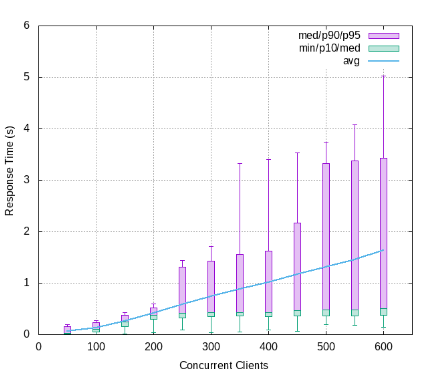
\includegraphics[scale=0.7]{figuras/benchmark1.png}
    \caption{Degradação no tempo de resposta. Fonte: ESPOSTE, 2017.}
  \label{fig:benchmark1}
\end{figure}

No primeiro experimento, clientes ficaram em um laço de repetição enviando
dados por requisições síncronas durante 4 minutos. O experimento foi feito
utilizando 11 diferentes configurações, variando o número de clientes
concorrentes. Com os resultados, que estão apresentados na Figura
\ref{fig:benchmark1}, pôde ser percebido que: (i) o microserviço
Resource Adaptor manteve o maior uso dos recursos, sendo considerado o
maior gargalo da plataforma, juntamente com o Data Collector, que também
apresentou uso intensivo da CPU; (ii) para 50 clientes concorrentes, o
tempo de resposta médio foi de 60 milissegundos; (iii) acima de 250 clientes
concorrentes, as requisições passaram a ter latência de 1 segundo
\cite{delesposte2017}.

\begin{figure}
  \centering
    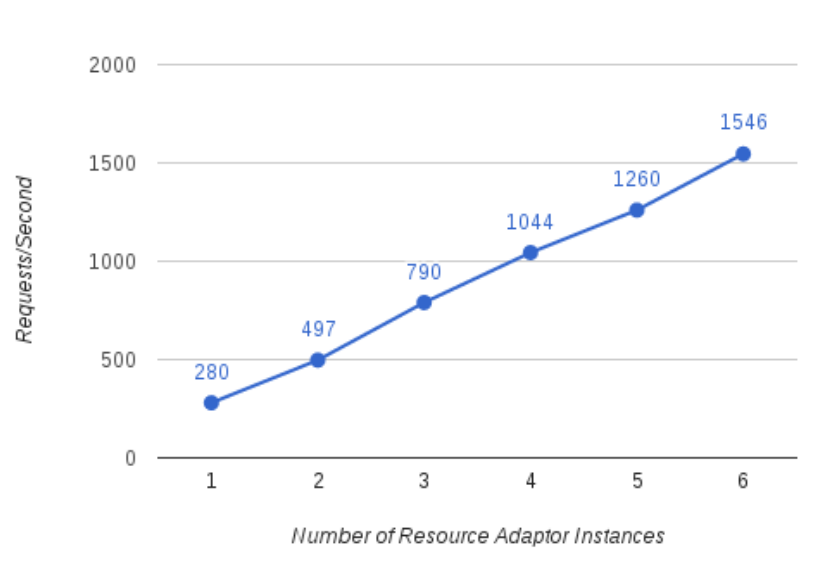
\includegraphics[scale=0.4]{figuras/benchmark2.png}
    \caption{Número de requisições por segundo com aumento de recursos. Fonte: ESPOSTE, 2017.}
  \label{fig:benchmark2}
\end{figure}

No segundo experimento, um cenário de 500 clientes concorrentes foi utilizado, 
durante 6 ciclos de 4 minutos, e com diferentes configurações de
\textit{hardware}, melhorando os recursos computacionais. Foi utilizado
balanceamento de carga igualitário (\textit{round-robin}) nos serviços
que foram identificados como os gargalos da plataforma - isto foi possível
graças aos princípios seguidos, mencionados anteriormente. Os resultados,
que estão apresentados na Figura \ref{fig:benchmark2}, permitem concluir que:
(i) só é necessário a melhora de alguns microserviços para melhor desempenho
da plataforma, até certo ponto; (ii) a plataforma consegue escalar linearmente
com a adição de recursos, o que mostra o quão escalável é o InterSCity. Além
disso, foi observado que, por conta do alto número de clientes, o RabbitMQ
passou a consumir grandes recursos, o que o trás como outro possível gargalo,
caso tenha disponível pouco recurso computacional \cite{delesposte2017}.

\chapter{PSEUDO-IMPLEMENTAÇÃO - ARQUITETURA LAMBDA}
\label{appendix:impl}

\section{CÓDIGO DA CAMADA BATCH}
\begin{python}
class BatchLayer(threading.Thread):
    daemon = True
    ...
    def run(self):
        heappush(hooks.actions, (10, Handler1.AcquireData))
        heappush(hooks.actions, (12, Handler2.AdjustDataModels))
        heappush(hooks.actions, (20, Handler3.ProcessData))
        heappush(hooks.actions, (21, Handler4.FindAnomalies))
        # extensible, new hooks can be added

        self.batch_view = sc.emptyRDD()

        while (True):
            # continuously processing
            rdd = spark.sql("SELECT * FROM sensor_data").cache()
                for op in hooks.actions:
                rdd = op(rdd).cache()
            self.batch_view = rdd # updates batch view
            rdd.unpersist()
            self.finished_batch = True # notifies speed layer
\end{python}

\section{CÓDIGO DA CAMADA SPEED}
\begin{python}
class SpeedLayer(threading.Thread):
    daemon = True
    ...
    def run(self):
        self.reset_realtime_view = False
        self.new_realtime_view = False

        def reset_realtime_view(stream):
            # checks if the batch layer finished its processing
            if (batch_view.finished_batch):
                batch_view.finished_batch = False
                stream.foreachRDD(lambda rdd: rdd.unpersist())
                self.reset_realtime_views = True
                return stream.filter(lambda a: false)
            else:
                return stream

        def notify_serving(stream):
            self.new_realtime_view = True

        # connects to Kafka
        kvs = KafkaUtils.createDirectStream(ssc, [topic], \\
            {"metadata.broker.list": brokers})

        heappush(hooks.actions, (10, Handler1.AcquireData))
        heappush(hooks.actions, (12, Handler2.AdjustDataModels))
        heappush(hooks.actions, (20, Handler3.ProcessData))
        heappush(hooks.actions, (21, Handler4.FindAnomalies))
        heappush(hooks.actions, (0xfffff, notify_serving))
        heappush(hook.actions, (0xffffff, lambda realtime_view: \
            reset_realtime_view(realtime_view)))

        self.realtime_view = kvs
        for op in hook.actions:
              # register hooks to be executed by the stream
              self.realtime_view = op(self.realtime_view)

        ssc.start() # start the stream
        ssc.awaitTermination()

\end{python}

\section{CÓDIGO DA CAMADA SERVING}
\begin{python}
class ServingLayer:
    ...
    def start(self):
        merged_data = sc.emptyRDD()
        speed_layer = SpeedLayer()
        batch_layer = BatchLayer()
        while (True):
            if (speed_layer.new_realtime_view):
                # updates results with available realtime views
                speed_layer.new_realtime_view = False
                merged_data = merged_data.union(\
                    speed_layer.realtime_view)
            if (speed_layer.reset_realtime_view):
                # reset realtime views when batches finishes
                merged_data = batch_layer.batch_view
                speed_layer.reset_realtime_view = False
            if (query):
                query(merged_data)
\end{python}

\end{apendicesenv}

